%CAPITULO 6
%pagina 23
\begin{frame}{Digresión: los valores exactos no importan}
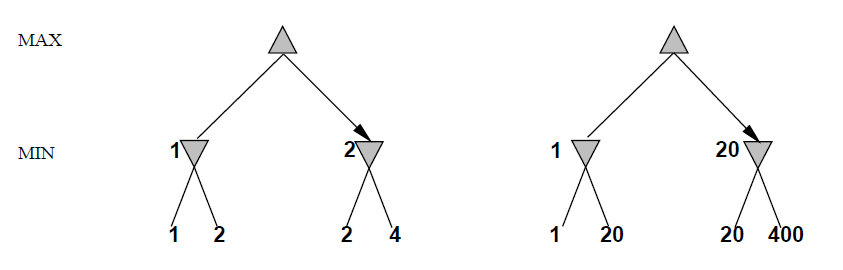
\includegraphics[scale=0.55]{images/23_image_cap6pag23.png}
El comportamiento se preserva bajo cualquier transformación \textcolor{red}{monotónica} de $EVAL$. \\
Solo importa el orden:\\
\hspace{1cm} Cuando la recompensa en los juegos deterministas actúa como una función de \textcolor{blue}{utilidad ordinal}.
\end{frame}